% SAPHIR — full journal manuscript draft (v0.1)
% Target: JAAMAS. Compile: pdflatex main.tex (twice).
\documentclass[11pt]{article}
\usepackage[margin=1in]{geometry}
\usepackage{booktabs}
\usepackage{graphicx}
\usepackage{hyperref}
\usepackage{tikz}
\usetikzlibrary{arrows.meta}
\title{SAPHIR: Secure Acoustic Pairing for Heterogeneous Inter-agent Rendezvous}
\author{Rathod Vaibhav Vishwas Ram\\{\small Department of Computer Science and Engineering, R.~V.~College of Engineering, Bengaluru, India}\\\small\texttt{github.com/vaibhav-rm/SAPHIR}}
\date{\small Manuscript draft v0.1 --- October 2026}
\begin{document}
\maketitle

\begin{abstract}
Voice AI agents that encounter each other on a call still converse the wasteful
way --- speech~$\to$~text~$\to$~LLM~$\to$~speech on both sides --- even though
both endpoints are machines. The viral Gibberlink demonstration (February 2025)
showed two agents switching to data-over-sound tones instead, but its switch is
unauthenticated, unnegotiated, unstructured, and opaque to human operators.
Meanwhile the emerging interoperability stack (MCP, A2A/ACP, ANP, InterSAGE)
uniformly assumes IP connectivity over HTTPS, leaving voice-only calls, PSTN
trunks, RF-restricted and offline settings without a pairing story. This paper
presents SAPHIR, a minimal authenticated pairing protocol for two heterogeneous
agents that share nothing but a bare audio channel: a three-phase handshake
(HELLO~$\to$~WELCOME~$\to$~KEY1~$\to$~KEY2) with ephemeral X25519 keys, compact
CBOR task encoding, ChaCha20-Poly1305 authenticated messaging, an optional
stop-and-wait ARQ layer for lossy acoustics, and a human-readable sidecar audit
log. An open prototype ($\sim$1.6k lines of Python including tests and harnesses) demonstrates a hotel-booking
dialogue end to end: 117--139\,B task frames across two domains, blocked spoof/replay/downgrade
attacks, 100\% pairing success on clean channels, 95--100\% under bursty
VoIP-like loss where raw frames score 0\%, and immediate cost breakeven that
widens to $\sim$65$\times$ at 20 turns. We state precisely what is measured,
what is modeled, and what remains --- over-air validation, PKI-backed identity,
and group sessions --- and close with open research questions.
\end{abstract}

\section{Introduction}
In February 2025 a hackathon project called Gibberlink~\cite{gibberlink}
demonstrated two ElevenLabs voice agents on a phone call discovering both sides
are AI and switching from English to \texttt{ggwave}~\cite{ggwave}
data-over-sound tones. The video passed 15\,M views and the intuition is sound:
rendering speech for a machine listener wastes two neural speech passes and
thousands of tokens per turn. The implementation, however, is a prompt (``switch
if the other side is AI'') plus raw tones. Four gaps follow directly: (1) the
switch is \emph{unauthenticated} --- any speaker can emit beeps; (2) the format
is \emph{unnegotiated} --- both sides must hardcode the same profile; (3) the
content is \emph{unstructured English} --- tones carry sentences, not intents;
(4) the exchange is \emph{opaque to humans} --- operators cannot read what was
agreed. A recorded beep replays; a crafted beep injects; a legacy peer is
silently beeped at.

In parallel, 2024--26 produced the first serious agent-interoperability stack:
Anthropic's MCP for agent-to-tool access, Google's A2A (now Linux Foundation)
for task delegation via Agent Cards, IBM/Cisco ACP variants for performative
messaging, ANP for decentralized discovery with W3C DIDs, and InterSAGE as the
identity/trust substrate~\cite{interop-survey,intersage}. Security analysis is
maturing alongside: A2ASecBench~\cite{a2asecbench} and ASB systematize
protocol-logic attacks that bypass default safeguards, and communication-graph
analysis~\cite{graphmeta} shows even encrypted transports leak
who-talks-to-whom. Yet every protocol in this stack assumes URL-addressable
agents over HTTP(S). IETF framework drafts~\cite{ietf-agents} list discovery,
negotiation, and fallback among open requirements. None answers: \emph{what if
the only shared channel is sound?} Near-term agent telephony (AI receptionists,
AI assistants calling businesses), PSTN trunks that destroy ultrasound,
RF-restricted facilities, and offline/disaster settings all produce voice-only
encounters between heterogeneous agents.

\textbf{Contribution.} We argue acoustic pairing deserves first-class protocol
status and present SAPHIR (Secure Acoustic Pairing for Heterogeneous
Inter-agent Rendezvous): detect, negotiate, encrypt, collaborate in structured
intents, and account for every exchange in a human-readable sidecar. We
contribute (i) the protocol (handshake, compact encoding, AEAD messaging,
optional ARQ); (ii) an explicit threat model with verified blocks; (iii) an
open prototype with seven evaluation harnesses; and (iv) a disciplined
measured-vs-modeled accounting that states exactly what is (and is not)
claimed. All artifacts are public to enable red-teaming.

\section{Background and related work}
\emph{Gibberlink and ggwave.} Gibberlink~\cite{gibberlink} contributes the
core observation (speech is wasteful machine-to-machine) and a demo, not a
protocol: no framing beyond ggwave frames, no handshake, no security.
\texttt{ggwave}~\cite{ggwave} is a data-over-sound modem (FSK + Reed-Solomon,
tens of bytes/sec in robust audible profiles) in the lineage of dial-up
modems; SAPHIR treats it as a byte pipe and adds everything above it.

\emph{The HTTP interop stack.} The four-protocol survey~\cite{interop-survey}
(MCP/ACP/A2A/ANP) proposes a phased roadmap from tool access to decentralized
agent marketplaces --- all over IP. InterSAGE~\cite{intersage} supplies the
missing trust substrate (persistent identity, capability-aware discovery,
attenuated delegation, audit trails) and explicitly complements, rather than
replaces, transport protocols. SAPHIR's claim is narrow and compatible: it is
the pairing layer for the one transport the stack omits, and its ephemeral-DID
handshake is designed to upgrade to InterSAGE-style credentials where IP exists
(hybrid mode).

\emph{Attack literature.} A2ASecBench~\cite{a2asecbench} taxonomizes
supply-chain and protocol-logic attacks across A2A stages; ASB benchmarks
prompt-injection, memory poisoning, and backdoors across agent backbones; both
find high attack success against default configurations. Our threat model
imports their methodology (named attacker capabilities, verified blocks) at the
acoustic layer, where the cheapest attacks --- replay and injection --- need
only a speaker.

\emph{Semantics and metadata.} Two recent critiques shape our design:
well-formed JSON does not imply shared meaning~\cite{semalign}, motivating our
ontology-tagged intent slots over raw English; and encrypted content still
exposes the communication graph, whose action-coupled metadata threatens
workflow integrity~\cite{graphmeta}, motivating our sidecar's selective
disclosure as future work rather than a solved claim.

\emph{Deployment context.} Industry surveys report the trust gap blocking
agentic-AI production (85\% exploring, 5\% in production)~\cite{ciscotrust};
IETF drafts~\cite{ietf-agents} formalize the missing negotiation/fallback
machinery. SAPHIR targets exactly that intersection for voice-only encounters.

\section{Problem and threat model}
Two heterogeneous voice agents share a low-bandwidth ($\sim$30\,Bps reference),
possibly lossy, possibly adversary-observable audio channel, plus optionally an
IP side channel (hybrid mode). Goals: pair within seconds, agree on codecs and
a task ontology, communicate confidentially with integrity, degrade explicitly
(never silently) with legacy peers, and leave a human-inspectable record.
Attacker capabilities: observe, record, replay, and emit arbitrary audio;
impersonate without keys; force or suppress the switch. Out of scope in this
version: attackers holding stolen session keys (needs PKI rotation),
traffic-analysis resistance, and denial-of-service on the acoustic medium.

\section{The SAPHIR protocol}
\textbf{Framing.} Length-prefixed CBOR envelopes,
\texttt{u32be len $\parallel$ CBOR(\{v,type,seq,sender,nonce,payload\})}, cap
200\,B (enforced). \textbf{Handshake.} HELLO (ephemeral \texttt{did:key},
codec/mode lists) $\to$ WELCOME (selected codec; peers offering no SAPHIR
codec are flagged and kept in English) $\to$ KEY1/KEY2 (32\,B X25519 ephemeral
pubkeys each way; HKDF-SHA256 derives a 32\,B ChaCha20-Poly1305 session key;
forward secrecy per pairing). \textbf{Messaging.} TASK/RESULT carry
\texttt{ChaCha(cbor(\{intent,slots,ontology,ts\}))} with the sender as AAD;
replays are rejected by sequence plus (nonce, ciphertext) sets.
\textbf{Compact encoding.} Hotel-ontology shorts (\texttt{hotel.book}$\to$\texttt{hb},
\texttt{date}$\to$\texttt{d}, \dots) cut task frames 182/202\,B $\to$ 117--139\,B
across hotel and taxi domains (non-default ontology tagged, value shorts);
legacy full-form still decodes. \textbf{ARQ (optional).} Stop-and-wait layer:
$\leq$110\,B CRC32 chunks (each fits one audible frame) with ACKs and bounded
retries, tick-driven and deterministic. \textbf{Audit.} Every frame is appended
to a JSONL sidecar with a human summary and decrypted view.
Figure~\ref{fig:hs} summarizes the exchange.

\begin{figure}[h]
\centering
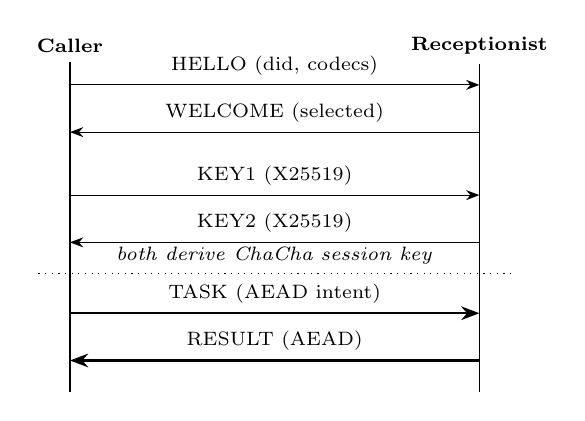
\begin{tikzpicture}[font=\scriptsize, >=Stealth]
\node (A) at (0,0) {\textbf{Caller}};
\node (B) at (5.2,0) {\textbf{Receptionist}};
\draw (A) -- (0,-4.4); \draw (B) -- (5.2,-4.4);
\draw[->] (0,-0.5) -- (5.2,-0.5) node[midway,above] {HELLO (did, codecs)};
\draw[->] (5.2,-1.1) -- (0,-1.1) node[midway,above] {WELCOME (selected)};
\draw[->] (0,-1.9) -- (5.2,-1.9) node[midway,above] {KEY1 (X25519)};
\draw[->] (5.2,-2.5) -- (0,-2.5) node[midway,above] {KEY2 (X25519)};
\draw[dotted] (-0.4,-2.9) -- (5.6,-2.9) node[above,midway] {\textit{both derive ChaCha session key}};
\draw[->,thick] (0,-3.4) -- (5.2,-3.4) node[midway,above] {TASK (AEAD intent)};
\draw[->,thick] (5.2,-4.0) -- (0,-4.0) node[midway,above] {RESULT (AEAD)};
\end{tikzpicture}
\caption{SAPHIR pairing. Negotiation is plaintext; tasks are encrypted; every frame is sidecar-logged.}
\label{fig:hs}
\end{figure}

\section{Implementation}
The prototype (\url{github.com/vaibhav-rm/SAPHIR}, MIT) is $\sim$1.6k lines of
Python: \texttt{protocol} (envelopes), \texttt{session} (handshake state
machine), \texttt{crypto} (X25519/HKDF/ChaCha), \texttt{codec} (compact maps),
\texttt{channel} (in-memory, lossy, burst-error, ARQ link), \texttt{agents}
(rule-based hotel and taxi tasks), \texttt{audit}, \texttt{metrics}. Seven harnesses
(\texttt{demo}, \texttt{bench}, \texttt{attacks}, \texttt{robustness},
\texttt{reliability}, \texttt{codec\_profiles}, \texttt{amortization}) plus 16
pytest tests cover functionality, attacks, and all sweeps. No audio hardware,
API keys, or network are required; channels are in-process byte pipes with
documented seeds.

\section{Evaluation}
\emph{Functionality.} Full pairing plus a two-intent booking dialogue runs end
to end; measured sizes: handshake 609\,B one-time, HELLO $\sim$194\,B,
KEY $\sim$107--113\,B, all four TASK frames 117--139\,B compact (hotel and
taxi domains), RESULT 126--139\,B.

\emph{Attacks (Table~\ref{tab:threat}).} A keyless attacker is rejected
(\texttt{InvalidTag}); exact replays are rejected (sequence reuse); legacy
peers are kept in English with an explicit flag. All three ship as failing-closed
checks in \texttt{evals/attacks.py}.

\begin{table}[h]
\centering\small
\caption{Threat outcomes: raw tones vs.\ SAPHIR (prototype-verified).}
\label{tab:threat}
\begin{tabular}{@{}lll@{}}
\toprule
Attack & Raw tones & SAPHIR \\
\midrule
Tone spoof / injection & succeeds & blocked (AEAD tag) \\
Replay of valid frame & succeeds & blocked (seq + nonce set) \\
Forced downgrade & silent & flagged, stays in English \\
Eavesdropping & plaintext & ciphertext \\
Stolen session keys & n/a & out of scope (needs PKI) \\
Who-talks-to-whom & n/a & out of scope \\
\bottomrule
\end{tabular}
\end{table}

\emph{Raw-channel sweep (50 trials/cell, no retransmission):} 100\% clean,
94\% at 1\% loss, 44\% at 10\% loss; corruption cliff (36\% at 0.1\%,
0\% at 0.5\%) since AEAD must reject forgeries --- integrity over
availability, by design. \emph{ARQ sweep (20 trials/cell,
Table~\ref{tab:arq}):} the same grid converts the cliff into retry cost:
100\%/95\% where raw scored 0\%, at $\sim$1.6$\times$ wire bytes; residual
10\%-loss failures are bounded-budget retry exhaustion.

\begin{table}[h]
\centering\small
\caption{ARQ vs.\ raw success rate per grid cell (drop, corruption).}
\label{tab:arq}
\begin{tabular}{@{}llll@{}}
\toprule
Cell & Raw & ARQ & Median retries (ARQ) \\
\midrule
(0.00, 0.000) & 100\% & 100\% & 0 \\
(0.05, 0.000) & 70\% & 100\% & 1 \\
(0.00, 0.005) & 0\% & 100\% & 8 \\
(0.05, 0.005) & 0\% & 95\% & 12 \\
(0.10, 0.000) & 44\% & 85\% & 3 \\
\bottomrule
\end{tabular}
\end{table}

\emph{Codec/noise profiles (byte-level burst models, 20 trials):}
clean 100\%, cafe-noise 95\%, bursty VoIP-like 95\%, harsh narrowband 80\% ---
bounding the design's operating envelope; waveform/over-air measurement is
explicitly future work. \emph{Amortization (Fig.~\ref{fig:amort}):} the 609\,B
handshake amortizes over turns (mean 263\,B wire per pair); modeled neural-cost
breakeven is immediate and $\sim$65$\times$ at 20 turns. Wall-clock is
deliberately not claimed: narrowband audio moves fewer bytes/sec than speech,
so SAPHIR trades time for near-zero neural compute; wire bytes stay above
raw-text-over-tones (structure plus auth tags), shown, not hidden.

\begin{figure}[h]
\centering
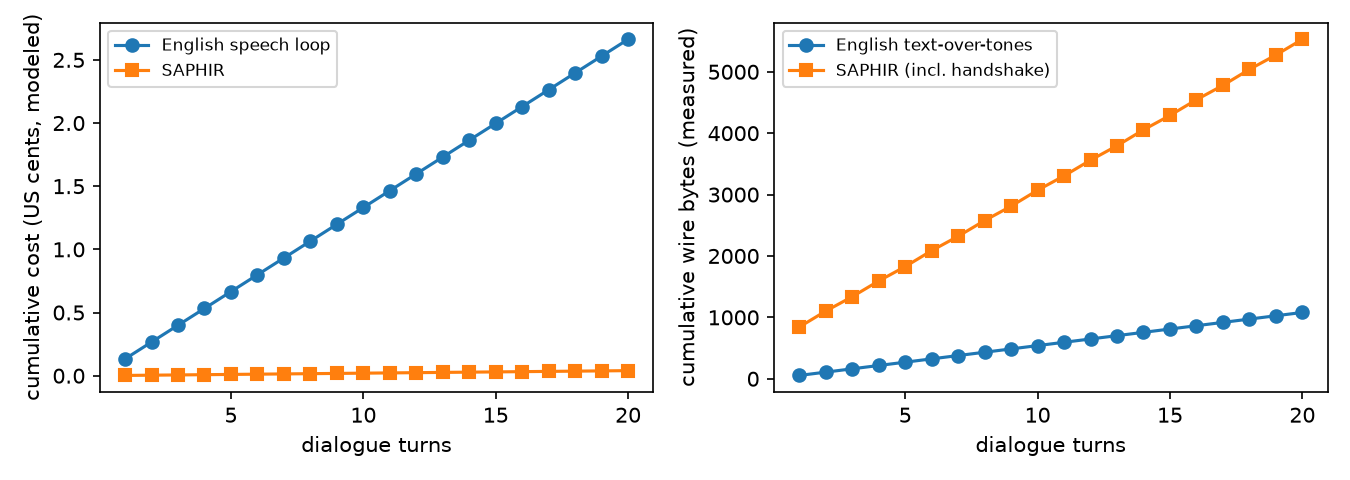
\includegraphics[width=\columnwidth]{../figures/amortization.png}
\caption{Cumulative modeled cost (left) and measured wire bytes (right) vs.\ dialogue turns. Cost wins immediately; bytes do not --- by design and on the record.}
\label{fig:amort}
\end{figure}

\section{Limitations and open questions}
(1) No over-air validation yet --- all loss models are byte-level; real
Opus/G.711 traces and room measurements are the next experiment. (2) Identity
is ephemeral, not PKI-backed; upgrading the HELLO to verifiable credentials
(where IP exists) is designed but unbuilt. Hand dictionaries are demo-scale;
schema-driven dictionaries negotiated in HELLO are the scalable compression
story and remain future work. (3) Two-party only; MLS-style groups
are future work. (4) Auditing stops at readability; selective disclosure
without workflow-graph leakage~\cite{graphmeta} is open. We invite red-teamers:
the artifact reproduces every table from one command each (see
\texttt{docs/REPRODUCIBILITY.md}).

\section{Conclusion}
Gibberlink asked the right question --- why speak to machines in speech? ---
and gave a demo answer. SAPHIR gives a protocol answer for the channels the
interop stack forgot: negotiate briefly, encrypt cheaply, speak in structure,
and keep every beep readable. The evidence here is preliminary but exact about
its boundaries; the operating envelope, the cost curves, and the open
challenges are published alongside the code so the community can push past
them.

\begin{thebibliography}{9}
\bibitem{gibberlink} B.~Starkov and A.~Pidkuiko. GibberLink, 2025. \texttt{github.com/PennyroyalTea/gibberlink}.
\bibitem{ggwave} G.~Gerganov. ggwave: data-over-sound library. \texttt{github.com/ggerganov/ggwave}.
\bibitem{interop-survey} A.~Ehtesham et al. A survey of agent interoperability protocols: MCP, ACP, A2A, and ANP. arXiv:2505.02279, 2025.
\bibitem{intersage} Z.~Zou et al. InterSAGE: the secure and verifiable interoperability protocol for an internet of agents. arXiv:2608.13030, 2026.
\bibitem{a2asecbench} T.~Li et al. A2ASecBench: a protocol-aware security benchmark for agent-to-agent multi-agent systems. ICLR, 2026.
\bibitem{graphmeta} B.~Dangol. From privacy to workflow integrity: communication-graph metadata in autonomous agent interoperability. arXiv:2606.07150, 2026.
\bibitem{semalign} Beyond message passing: toward semantically aligned agent communication. arXiv:2604.02369.
\bibitem{ietf-agents} J.~Rosenberg. Framework, use cases and requirements for AI agent protocols. IETF draft-rosenberg-ai-protocols, 2025; Y.~Cui. Cross-domain interoperability framework. draft-cui-dmsc-agent-cdi, 2026.
\bibitem{ciscotrust} Cisco. The agent trust gap: what our research reveals about agentic AI security. 2026.
\end{thebibliography}
\end{document}
